\section{图幅与比例}
在\ref{sec:zhoushitu}节中,我们将图纸尺寸设置为ISO A4(210.00x297.00毫米),视口的显示比例设置成了5:1。之所以这样设置,其目的是确保使用的图纸和比例都符合国家制定的制图标准。因此本节将介绍图纸幅面和比例相关的国家标准。
\subsection{图纸幅面与格式}
\subsubsection{图纸幅面}
图纸幅面是指整张图纸的尺寸大小。工程中为了便于图纸的装订、保管及合理利用图纸,要求图纸幅面大小要符合表\ref{tab:tuzhifumian}的规定。
\begin{table}[htbp]
\caption{图纸幅面}\label{tab:tuzhifumian}
\begin{tabu}to \linewidth {X[cm]*5{|X[cm]}}
\tabucline -
幅面代号&A0&A1&A2&A3&A4\\
\tabucline -
$B\times L$&$841\times 1189$&$594\times 841$& $420\times 594$&$297\times 420$&$210\times 297$\\
\tabucline -
$e$&\multicolumn{2}{c|}{20}&\multicolumn{3}{c}{10}\\
\tabucline -
$c$&\multicolumn{3}{c|}{10}&\multicolumn{2}{c}{5}\\
\tabucline -
$a$&\multicolumn{5}{c}{25}\\
\tabucline -
\tabuphantomline
\end{tabu}
\end{table}

\begin{figure}[htbp]
\centering
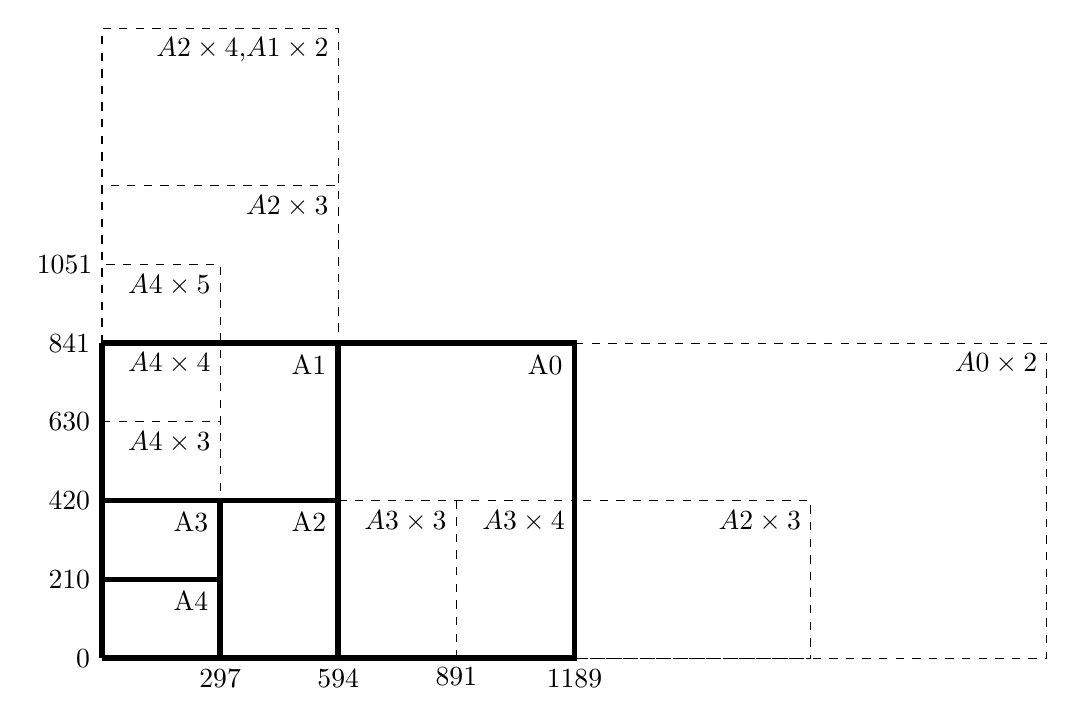
\begin{tikzpicture}
\draw[line width=0.7mm] (0,0)node[left]{0}--(0,1cm)node[left]{210}--(0,2cm)node[left]{420}--(0,3cm)node[left]{630}--(0,4cm)node[left]{841};
\draw[dashed](0,4cm)--(0,5cm)node[left]{1051}--(1.5cm,5cm)node[below left]{$A4\times 5$}--(1.5cm,2cm);
\draw[line width=0.7mm](0,1cm)--(1.5cm,1cm)node[below left]{A4}(0,2cm)--(1.5cm,2cm)node[below left]{A3}--(1.5cm,0)node[below]{297};
\draw[dashed](0,3cm)--(1.5cm,3cm)node[below left]{$A4\times 3$};
\draw[line width=0.7mm](0,4cm)--(3cm,4cm)node[below left]{A1}--(3cm,0)node[below]{594}(1.5cm,2cm)--(3cm,2cm)node[below left]{A2};
\draw[line width=0.7mm](3cm,4cm)--(6cm,4cm)node[below left]{A0}--(6cm,0)node[below]{1189}--(0,0);
\draw[dashed](3cm,2cm)--(4.5cm,2cm)node[below left]{$A3\times 3$}--(6cm,2cm)node[below left]{$A3\times 4$}(4.5cm,2cm)--(4.5cm,0)node[below]{891};
\draw[dashed](1.5cm,4cm)node[below left]{$A4\times 4$};
\draw[dashed](0,4cm)rectangle (3cm,6cm)node[below left]{$A2\times 3$};
\draw[dashed](6cm,0)rectangle (9cm,2cm)node[below left]{$A2\times 3$};
\draw[dashed](0,4cm)rectangle (3cm,8cm)node[below left]{$A2\times 4$,$A1\times 2$};
\draw[dashed](6cm,0)rectangle (12cm,4cm)node[below left]{$A0\times 2$};
\end{tikzpicture}
\caption{图纸幅面及加长边} \label{fig:tufujiachang}
\end{figure}
\subsubsection{图框}


\tikzset{
>=latex,
center lines/.style={dash pattern=on 20pt off 3pt on 2pt off 3pt},
importance lines/.style={line width=1pt}
}
\begin{figure}[htbp]
\centering
\subfloat[留装订边格式]{
\begin{tikzpicture}
\draw(0,0)rectangle(4cm,5cm);
\draw[line width=0.7mm](0.5cm,0.25cm)rectangle(3.75cm,4.75cm)(1.5cm,0.25cm)--(1.5cm,1cm)--(3.75cm,1cm)node[midway,below]{标题栏};
\draw(-0.7cm,0)--(0,0)(-0.7cm,5cm)--(0cm,5cm);
\draw[<->](-0.5cm,0)--(-0.5cm,5cm)node[midway,above,rotate=90]{$L$};
\draw(0,-0.7cm)--(0,0)(4cm,-0.7cm)--(4cm,0);
\draw[<->](0,-0.5cm)--(4cm,-0.5cm)node[midway,above]{$B$};
\draw[->](1cm,-0.45cm)--(1cm,0);
\draw[->](1cm,0.65cm)--(1cm,0.25cm)node[midway,above,rotate=90]{$c$};
\draw(1cm,0)--(1cm,0.25cm);
\draw[->](-0.4cm,2cm)--(0,2cm);
\draw[->](0.9cm,2cm)--(0.5cm,2cm);
\draw(0,2cm)--(0.5cm,2cm)node[midway,above]{$a$};
\draw[->](2cm,5cm)--(2cm,4.35cm)--(2cm,4.75cm);
\draw[->](2cm,5.45cm)--(2cm,5cm)node[midway,above,rotate=90]{$c$};
\draw[->](4cm,2.5cm)--(3.3cm,2.5cm)--(3.75cm,2.5cm);
\draw[->](4.45cm,2.5cm)--(4cm,2.5cm)node[midway,above]{$c$};

\begin{scope}[xshift=5.5cm]
\draw(0,0)rectangle(7cm,5cm);
\draw[line width=0.7mm](0.5cm,0.25cm)rectangle(6.75cm,4.75cm)(4.5cm,0.25cm)--(4.5cm,1cm)--(6.75cm,1cm)node[midway,below]{标题栏};
\draw(-0.7cm,0)--(0,0)(-0.7cm,5cm)--(0cm,5cm);
\draw[<->](-0.5cm,0)--(-0.5cm,5cm)node[midway,above,rotate=90]{$B$};
\draw(0,-0.7cm)--(0,0)(7cm,-0.7cm)--(7cm,0);
\draw[<->](0,-0.5cm)--(7cm,-0.5cm)node[midway,above]{$L$};
\draw[->](3cm,-0.45cm)--(3cm,0);
\draw[->](3cm,0.65cm)--(3cm,0.25cm)node[midway,above,rotate=90]{$c$};
\draw(3cm,0)--(3cm,0.25cm);
\draw[->](-0.4cm,2cm)--(0,2cm);
\draw[->](0.9cm,2cm)--(0.5cm,2cm);
\draw(0,2cm)--(0.5cm,2cm)node[midway,above]{$a$};
\draw[->](3.5cm,5cm)--(3.5cm,4.35cm)--(3.5cm,4.75cm);
\draw[->](3.5cm,5.45cm)--(3.5cm,5cm)node[midway,above,rotate=90]{$c$};
\draw[->](7cm,2.5cm)--(6.3cm,2.5cm)--(6.75cm,2.5cm);
\draw[->](7.45cm,2.5cm)--(7cm,2.5cm)node[midway,above]{$c$};
\end{scope}
\end{tikzpicture}}

\subfloat[不留装订边格式]{
\begin{tikzpicture}
\draw(0,0)rectangle(4cm,5cm);
\draw[line width=0.7mm](0.25cm,0.25cm)rectangle(3.75cm,4.75cm)(1.5cm,0.25cm)--(1.5cm,1cm)--(3.75cm,1cm)node[midway,below]{标题栏};
\draw(-0.7cm,0)--(0,0)(-0.7cm,5cm)--(0cm,5cm);
\draw[<->](-0.5cm,0)--(-0.5cm,5cm)node[midway,above,rotate=90]{$L$};
\draw(0,-0.7cm)--(0,0)(4cm,-0.7cm)--(4cm,0);
\draw[<->](0,-0.5cm)--(4cm,-0.5cm)node[midway,above]{$B$};
\draw[->](1cm,-0.45cm)--(1cm,0);
\draw[->](1cm,0.65cm)--(1cm,0.25cm)node[midway,above,rotate=90]{$c$};
\draw(1cm,0)--(1cm,0.25cm);
\draw[->](-0.4cm,2cm)--(0,2cm);
\draw[->](0.65cm,2cm)--(0.25cm,2cm)node[midway,above]{$c$};
\draw(0,2cm)--(0.25cm,2cm);
\draw[->](2cm,5cm)--(2cm,4.35cm)--(2cm,4.75cm);
\draw[->](2cm,5.45cm)--(2cm,5cm)node[midway,above,rotate=90]{$c$};
\draw[->](4cm,2.5cm)--(3.3cm,2.5cm)--(3.75cm,2.5cm);
\draw[->](4.45cm,2.5cm)--(4cm,2.5cm)node[midway,above]{$c$};

\begin{scope}[xshift=5.5cm]
\draw(0,0)rectangle(7cm,5cm);
\draw[line width=0.7mm](0.25cm,0.25cm)rectangle(6.75cm,4.75cm)(4.5cm,0.25cm)--(4.5cm,1cm)--(6.75cm,1cm)node[midway,below]{标题栏};
\draw(-0.7cm,0)--(0,0)(-0.7cm,5cm)--(0cm,5cm);
\draw[<->](-0.5cm,0)--(-0.5cm,5cm)node[midway,above,rotate=90]{$B$};
\draw(0,-0.7cm)--(0,0)(7cm,-0.7cm)--(7cm,0);
\draw[<->](0,-0.5cm)--(7cm,-0.5cm)node[midway,above]{$L$};
\draw[->](3cm,-0.45cm)--(3cm,0);
\draw[->](3cm,0.65cm)--(3cm,0.25cm)node[midway,above,rotate=90]{$c$};
\draw(3cm,0)--(3cm,0.25cm);
\draw[->](-0.4cm,2cm)--(0,2cm);
\draw[->](0.65cm,2cm)--(0.25cm,2cm)node[midway,above]{$c$};
\draw(0,2cm)--(0.25cm,2cm);
\draw[->](3.5cm,5cm)--(3.5cm,4.35cm)--(3.5cm,4.75cm);
\draw[->](3.5cm,5.45cm)--(3.5cm,5cm)node[midway,above,rotate=90]{$c$};
\draw[->](7cm,2.5cm)--(6.3cm,2.5cm)--(6.75cm,2.5cm);
\draw[->](7.45cm,2.5cm)--(7cm,2.5cm)node[midway,above]{$c$};
\end{scope}
\end{tikzpicture}}
\caption{图框格式}\label{fig:zhuangding}
\end{figure}

\subsection{比例}
比例是图形与其实物相应要素的线性尺寸之比。线性尺寸是能够用直线表达的尺寸。例如圆弧的半径,直线的长度等。

通常图样的比例分为原值比例、放大比例和缩小比例三种。画图时应优先采用1:1的比例进行绘制,以便能够看出物体的真实大小。若无法采用1:1的比例时,则应优先选用表\ref{tab:biaozhunbili}中规定的比例系列,必要时也可采用表\ref{tab:biaozhunbili} 规定的比例系列。
\begin{table}[htbp]
\caption{标准比例系列}\label{tab:biaozhunbili}

\begin{tabu} to \linewidth {X[cm]|X[c m]|X[c m]|X[c m]}
\tabucline -
种\qquad 类&\multicolumn{3}{c}{ 比\qquad 例 } \\
\tabucline -
原始比例&\multicolumn{3}{c}{1:1}\\
\tabucline -
放大比例&
$\begin{tabu}{c}
2:1\\
2\times 10^n:1
\end{tabu}$
&
$\begin{tabu}{c}
5:1\\
5\times 10^n:1
\end{tabu}$
&$1\times 10^n$:1\\
\tabucline -
缩小比例&
$\begin{tabu}{c}
1:2\\
1:2\times 10^n
\end{tabu}$
&
$\begin{tabu}{c}
1:5\\
1:5\times 10^n
\end{tabu}$
&
$\begin{tabu}{c}
1:10\\
1:10\times 10^n
\end{tabu}$\\
\tabucline -
\tabuphantomline
\end{tabu}
\end{table}

\begin{table}[htbp]

\begin{tabu}to \linewidth {X[cm]|X[2cm]|X[cm]|X[cm]|X[2cm]}
\tabucline -
种\qquad 类&\multicolumn{4}{c}{比\qquad 例}\\
\tabucline -
放大比例&\multicolumn{2}{c|}{4:1\quad $4\times 10^n$:1}&\multicolumn{2}{c}{2.5:1\quad $2.5\times 10^n$:1}\\
\tabucline -
缩小比例&$\begin{tabu}{c}
1:3\\
1:3\times 10^n
\end{tabu}$
&
\multicolumn{2}{c|}{$\begin{tabu}{c}
1:4\\
1:4\times 10^n
\end{tabu}$}
&
$\begin{tabu}{c}
1:6\\
1:6\times 10^n
\end{tabu}$\\
\tabucline -
\tabuphantomline
\end{tabu}
\caption{比例系列}\label{tab:biaoxilei}
\end{table}



\endinput